\setcounter{figure}{0}

\section{14th May 2023: He is coming soon!}
\subsection*{Text: Revelation 22:6-16}
  \begin{quote}
    [6] And he said to me, “These words are trustworthy and true. And the
    Lord, the God of the spirits of the prophets, has sent his angel to show
    his servants what must soon take place.”

    [7] “And behold, I am coming soon. Blessed is the one who keeps the words
    of the prophecy of this book.”

    [8] I, John, am the one who heard and saw these things. And when I heard
    and saw them, I fell down to worship at the feet of the angel who showed
    them to me, [9] but he said to me, “You must not do that! I am a fellow
    servant with you and your brothers the prophets, and with those who keep
    the words of this book. Worship God.”

    [10] And he said to me, “Do not seal up the words of the prophecy of this
    book, for the time is near. [11] Let the evildoer still do evil, and the
    filthy still be filthy, and the righteous still do right, and the holy
    still be holy.”

    [12] “Behold, I am coming soon, bringing my recompense with me, to repay
    each one for what he has done. [13] I am the Alpha and the Omega, the
    first and the last, the beginning and the end.”

    [14] Blessed are those who wash their robes, so that they may have the
    right to the tree of life and that they may enter the city by the gates.
    [15] Outside are the dogs and sorcerers and the sexually immoral and
    murderers and idolaters, and everyone who loves and practices falsehood.

    [16] “I, Jesus, have sent my angel to testify to you about these things
    for the churches. I am the root and the descendant of David, the bright
    morning star.”
  \end{quote}
\subsection*{Notes}
\begin{itemize}
  \item{Since this is the last sermon on Revelation, here we have a recap of
  the entire letter:
  \begin{itemize}
    \item{Background of John's audience: living in Rome during the Roman
    empire, facing much persecution as well as bad influences from the
    surrounding culture. An example of persecution is matyrdom, and an
    example of bad influences would be how craftsmen were required to join a
    guild to sell their craftsware, and in those guild meetings there would
    be food sacrificed to idols and orgies.}
    \item{Hence, Revelation is a letter written to the christians back then
    to encourage them to be faithful even in the midst of persecution and
    their morally decadent society.}
    \item{How does Revelation encourage the saints? First, there is a vision
    of Christ in chapter 1, then there is the worship in heaven in chapters
    4-5, and then the bulk of the book is about the destruction of evil. The
    destruction of evil is a big part of the book because ultimately Satan,
    the evil one, is the one behind the persecutions of the Christians and
    also the moral decadence of the book. And lastly, after the
    encouragement, there is an exhortation to remain steadfast, even to
    choose martyrdom.}
    \item{The destruction of evil is the part that is subject to different
    interpretations. For example, some people read chapters $17-20$
    chronologically in a more literal, premillenial version. Other people
    read it in an idealist, amillenial fashion. True Way takes the latter
    view, where the $1000$ years is emblematic of the entire age between
    Christ's ascension and Christ's second coming. And as the ``day of the
    Lord'' comes, the evil will intensify. But at the end, all the battles
    written are just different panels of the same event, the great ``day of
    the Lord'', which is the culmination of the seventh scroll, the seventh
    trumpet and the seventh bowl, which signals the final defeat of evil. }
  \end{itemize}}
  \item{Our text today is the epilogue which concludes the letter. There are
  two main themes in the epilogue here. These two themes also appear in the
  prologue, and hence we have an inclusio structure here. The first theme is:
  ``I am coming soon'', and the second theme is: ``the words of the
  prophecy''. We can also find these two themes in the prologue (chapter 1).}
  \item{The first theme, ``I am coming soon''. $2000$ years have passed, and
  Christ has yet to come. Why? First, we must first remember God's
  perspective on time, as said in 2 Peter 3:8-9. Christ is delaying His
  coming because of His mercy. Second, the root word for soon here actually
  means quickly and suddenly, rather than $X$ years from now. Hence, Christ's
  words that ``He is coming soon'' is to summon us to preparedness. If we
  compare Revelation 22 with Daniel 12, we see that Daniel is supposed to
  seal up the words of the prophecy, but John was not supposed to. Hence,
  this tells us that the time is really near. }
  \item{The second theme, ``the words of the prophecy'' are trustworthy and
  true. Here, these words are given in the following order: God $\rightarrow$
  Jesus $\rightarrow$ Angel $\rightarrow$ John $\rightarrow$ saints. In fact,
  if we generalise this theme to the entire book of the Bible rather than
  just Revelation, then all of God's revelation in the Bible are trustworthy
  and true. We note that Genesis and Revelation actually form a big inclusio,
  with the common themes being the tree of life, human beings in God's
  presence. We also see Jesus the root, the descendent of David which is the fulfilment of Genesis 3:16-17. Since the entire testimony of God is trustworthy, hence, we are to keep God's word.}
  \item{To keep God's word, we receive it in faith, hold fast to it in hope,
  and live it out in love. The first and single most important in keeping
  God's Word is to worship Him. Not just on sunday, but in our lives through
  how we live. Compare this with the pattern of the world which is to worship
  self or to worship created things.}
  \item{John also says not to ``add or remove to the words of the prophecy''.
  Generaising this to beyond Revelation, we see that we must not cherry pick
  what we want to believe/obey (such as ignoring certain commandments like
  the commandment against homosexual activity (psleek's example) or divorce
  (my example)). We must also not pervert the Gospel
  (prospertity gospel). \KH{(My thoughts:) There needs to be some elaboration
  on the first point though because if not critics will also bring up how we
  also don't have head coverings for women. Clearly, some commandments are
  contextual; we do not interpret the commands for masters and slave as
  endorsing the institution of slavery. There needs to be a criteria given to
  say what is contextual or not, because critics can also argue that the
  commandments against homosexuality are just contextual. }}
  \item{The letter ends with an exhortation that God's grace is with us. Our whole Christian life, our obedience, is only possible through grace. }
  \item{\begin{figure}[H]
    \centering
    % 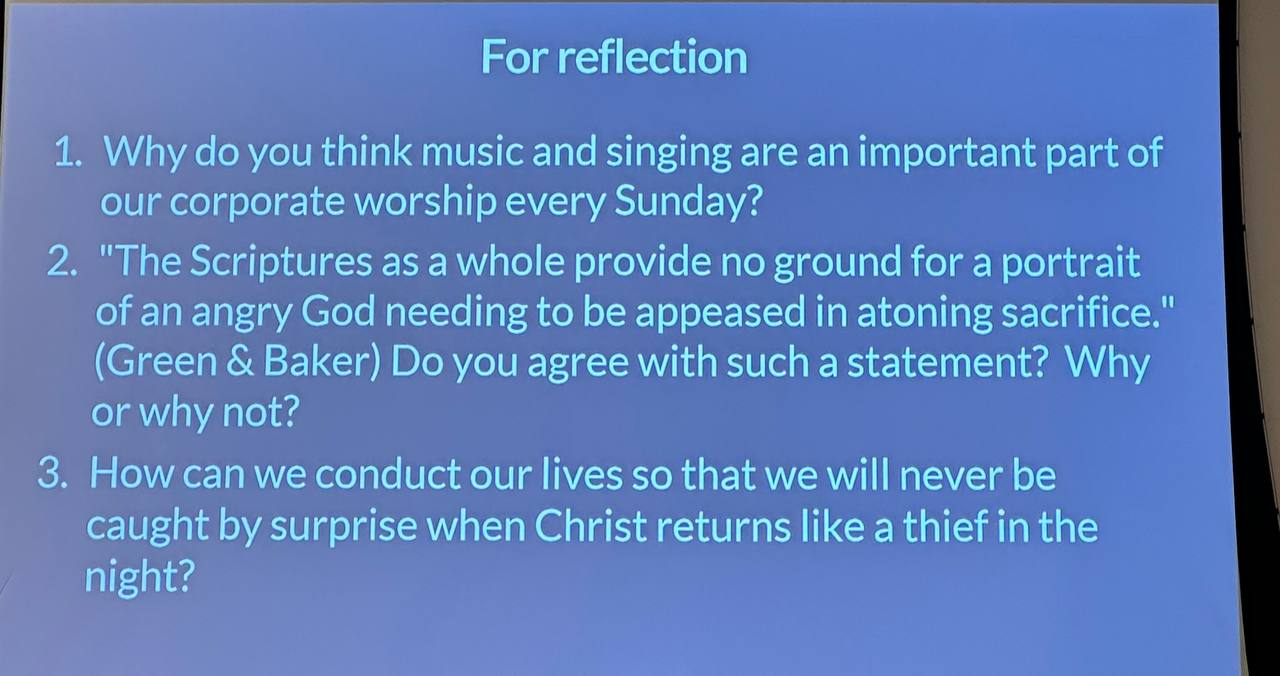
\includegraphics[width=0.8\textwidth, trim={0cm 0cm 0cm 0cm},clip]{Figures/marchSermon4Reflections.jpg}
    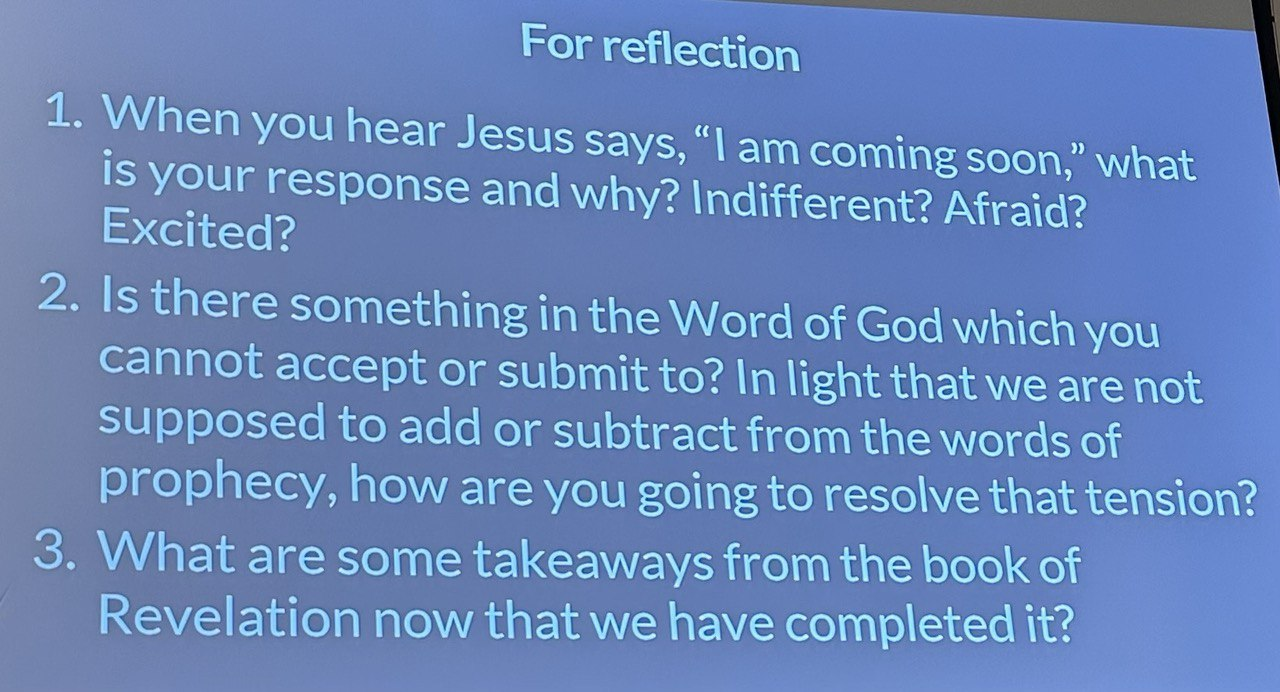
\includegraphics[width=0.8\textwidth, trim={0cm 0cm 0cm 0cm},clip]{Figures/maySermon2Reflections.jpg}
    \caption[]{Reflection questions for this sermon}
    \label{}
  \end{figure}}
\end{itemize}